\begin{figure*}
\centering
\begin{subfigure}[h]{\textwidth}
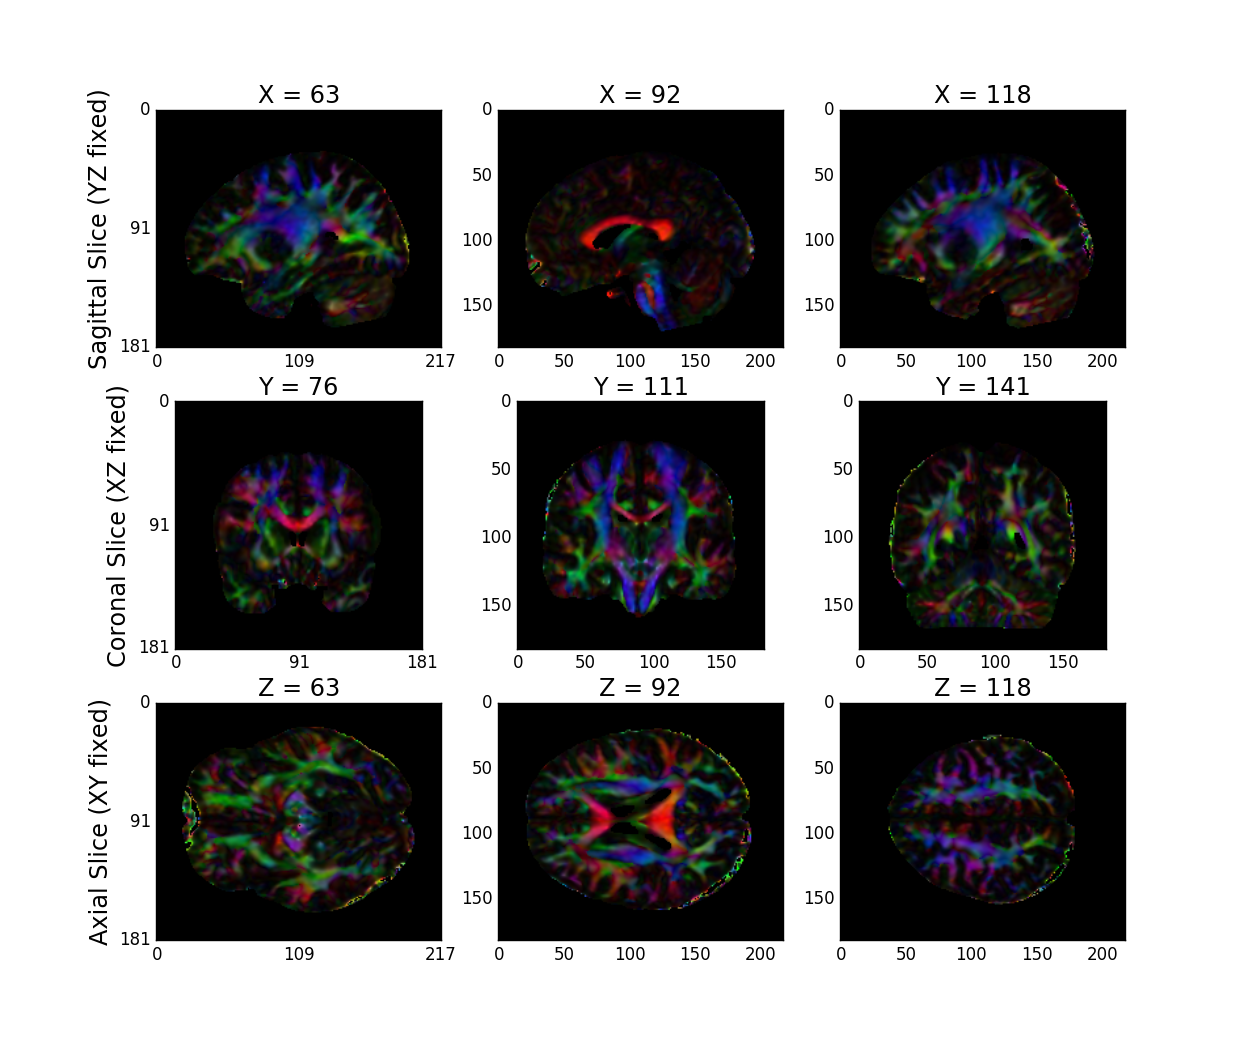
\includegraphics[width=0.9\textwidth]{./qa_figs/fig_dwi_tensors.png}
\end{subfigure}
\caption{\textbf{\ndmgd~Tensor Estimation QA}. \ndmgd~produces tensor QA showing the voxelwise determininstic tensor model fit to the aligned dMRI sequence.}
% @rjv: gk can't clarify much more than this is the default for VTK.
% @eb: then you can figure it out.  at a minimum explain the colors.  in previous plots you should have explained the different views, z-slices, and XY axes.
\label{fig:dMRI_tensor}
\end{figure*}